% Fucking default pgfsys-dvipdfmx.def screws up normal text, so use another driver
\def\pgfsysdriver{pgfsys-dvipdfm.def}
\documentclass[10pt, compress, usetitleprogressbar, protectframetitle]{beamer}

\usetheme{m}

\usepackage{pgfpages}
%\setbeamertemplate{note page}[plain]
\setbeameroption{show notes on second screen=right}

\usepackage{booktabs}

\usepackage{datetime}
%	\usepackage[scale=2]{ccicons}
%	\usepackage{minted}
%	\usepgfplotslibrary{dateplot}
%	\usemintedstyle{trac}

\usepackage{textpos}
% Fixes bad positioning of hats
\usefonttheme{professionalfonts}%[onlymath]{serif}
\usepackage{subcaption}
%\usepackage{epstopdf}
\usepackage{siunitx}
\usepackage{braket}

%%%%%%%%%%%%%%%%%%%%%%%%%%%%%%%%%%%%%%%%%%%%%%%%%%%%%%%%%%%
% datetime specific configuration                         %
%%%%%%%%%%%%%%%%%%%%%%%%%%%%%%%%%%%%%%%%%%%%%%%%%%%%%%%%%%%
\newdateformat{monthyear}{\monthname[\THEMONTH] \THEYEAR}

\graphicspath{{figures/PNG/}{figures/PDF/}{figures/}}

%\addtobeamertemplate{frametitle}{}{%
%\begin{textblock*}{1.5cm}(-0.7cm,0.7\textheight)
%
\includegraphics[height=1.5cm]{logo_unitn}
%\end{textblock*}}

\title{Variational Monte Carlo methods for quantum dots}
\subtitle{}
\date{\monthyear\today}
%\author{
\includegraphics[width=3cm]{logo_unitn}\\[0.25cm] Matteo Seclì}
\author{Matteo Seclì}
\institute{\scshape University of Trento -- Department of Physics}

%\logo{
\includegraphics[height=1cm]{logo_unitn}}

\begin{document}

\maketitle

\begin{frame}{Contents}
	\tableofcontents
\end{frame}

\section{What are quantum dots?}

\begin{frame}{Quantum dots as artificial atoms}

	\uncover<+->{Quantum dots can be thought as \alert{artificial atoms}.}
	
	\note{Like natural atoms, they are...}
	
	\uncover<+->{Similarities with natural atoms:}
	
	\begin{itemize}[<+->]
		\item They are made up of electrons confined in an \emph{attractive potential}
		\item They have a shell-structure with its relative \alert{magic numbers}
	\end{itemize}

	\uncover<+->{Differences:}
	
	\begin{itemize}[<+->]
		\item \emph{Shape} of the potential (2D isotropic harmonic potential)
		\item \emph{Dimensions} (quantum dots are a few hundred angstroms big)
		\item \emph{Structure} and source of the potential
	\end{itemize}
	
	\note{
		While in natural atoms the attractive potential is generated by a charged nucleus, in quantum dots there is no such a thing.
		
		To understand how the confinement is generated in this case, we have to take a look at the internal structure of such devices.
	}
	
\end{frame}

\begin{frame}{Structure}

	\uncover<+->{Building technique: stack up different layers of \alert{semiconductor} materials.}
	
	\uncover<+->{Then, an electron gas forms at the interface between two layers.}
	
	\uncover<+->{The electron gas is confined by applying an electric voltage to the whole structure, either laterally of vertically.}
	
	\uncover<+->{	
		\begin{figure}
			\begin{subfigure}[t]{0.5\textwidth}
				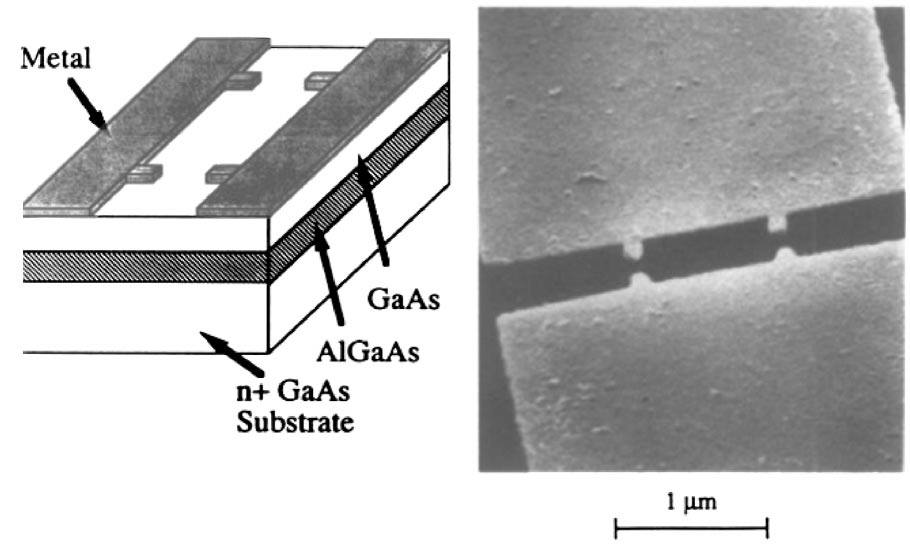
\includegraphics[width=\textwidth]{Figure_5_Reimann}
				\caption{Lateral quantum dot.}
		    \end{subfigure}
			\begin{subfigure}[t]{0.4\textwidth}
				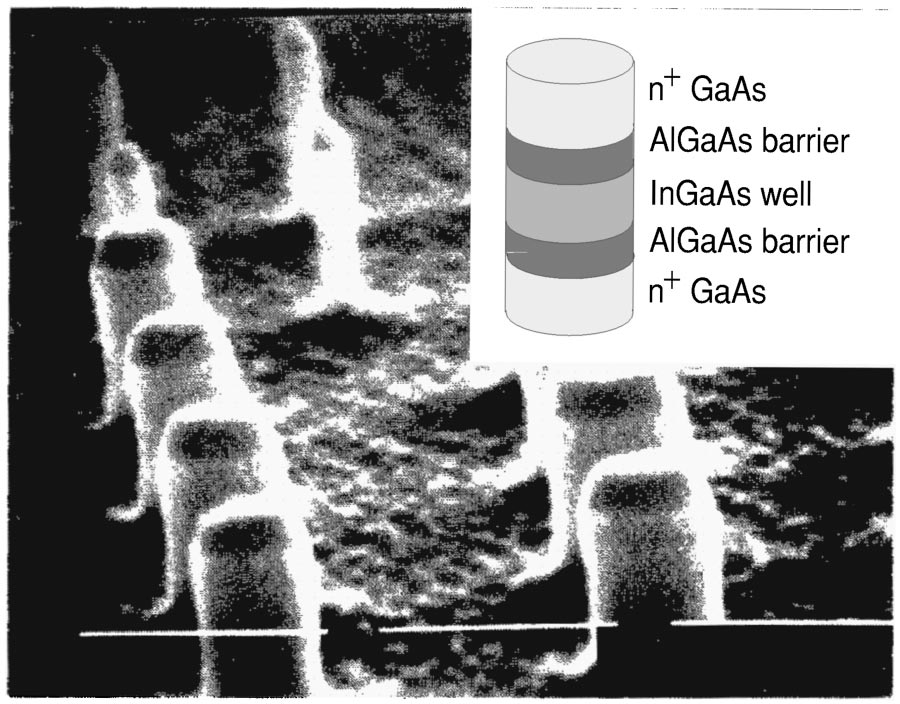
\includegraphics[width=\textwidth]{Figure_4_Reimann}
				\caption{Etched quantum dots.}
		    \end{subfigure}
		\end{figure}
	}
	
	\note{In the etched quantum dots figure, the white bars have a length of $\SI{0.5}{\micro\meter}$.}
	
\end{frame}

\begin{frame}{The single-electron transistor}

	\uncover<+->{A quantum dot can be schematized as a \emph{single-electron transistor}.}
	
	\uncover<+->{Its charge is a multiple of the elementary charge and transport proceeds one electron at the time.}
	
	\uncover<+->{
		\begin{figure}
			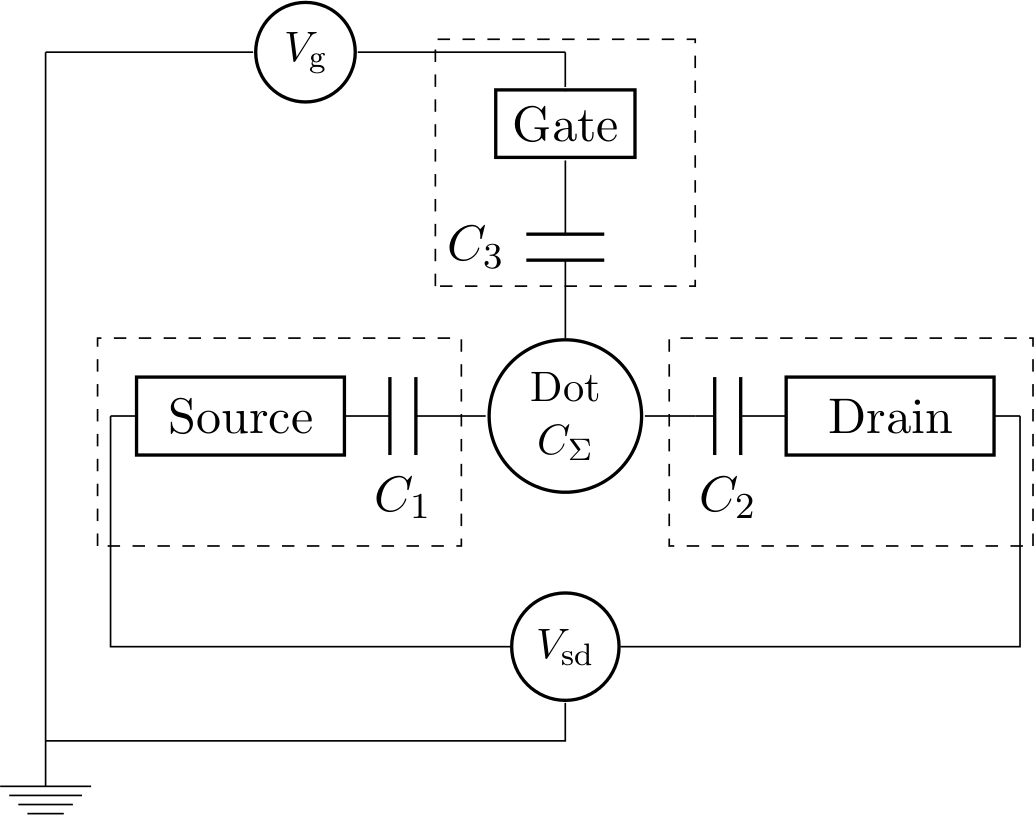
\includegraphics[width=0.6\textwidth]{SET}
		\end{figure}	
	}
	
	\note{In figure, scheme of a single electron transistor. The island has index 0, the source has index 1, the drain index 2 and the gate index 3. The capacitances are meant to be intrinsic capacitances of the respective electrode (source, drain or gate)}	
	
\end{frame}

\begin{frame}{The Coulomb blockade effect}

	\begin{itemize}[<+->]
		\item The electron island is weakly coupled with source and drain via tunnel barriers.
		\item When the thermal energy is not enough to make an electron tunnel the barriers, the conduction is blocked.
		\item This effect is called the \alert{Coulomb blockade}, and shows up in \emph{conductance} measurements.
	\end{itemize}
	
	\uncover<+->{
		\begin{figure}
			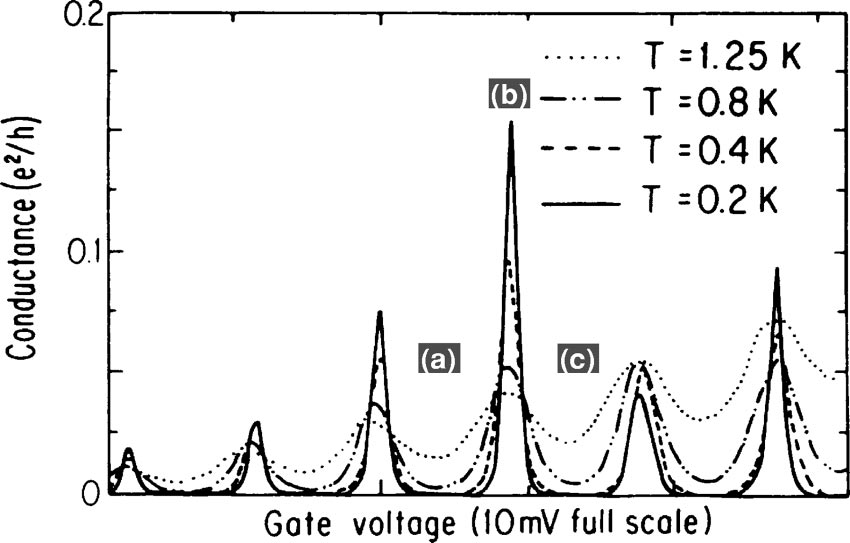
\includegraphics[width=0.6\textwidth]{Figure_6_Reimann}
		\end{figure}	
	}
	
	\note{In figure, Coulomb oscillations in a lateral quantum dot.}
	
\end{frame}

\begin{frame}{The Coulomb blockade effect}
	
	\begin{figure}
		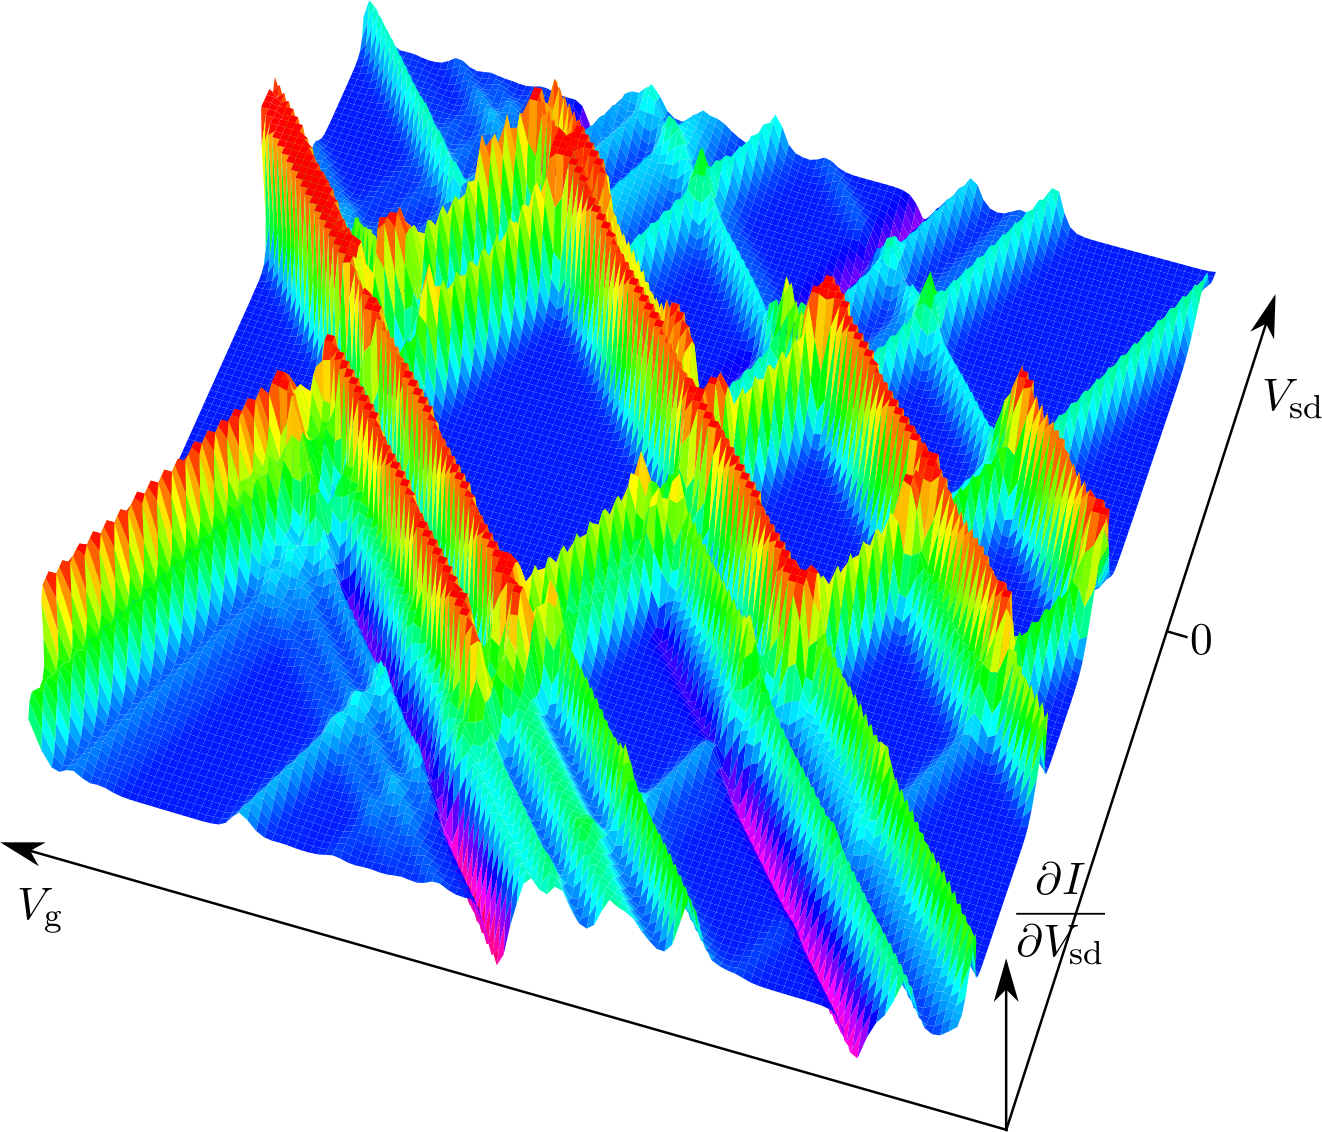
\includegraphics[width=0.6\textwidth]{diff_cond}
		\caption{Differential conductance measurements in a nanowire.}
	\end{figure}	
	
\end{frame}

\begin{frame}{Band diagram}

	\begin{figure}
		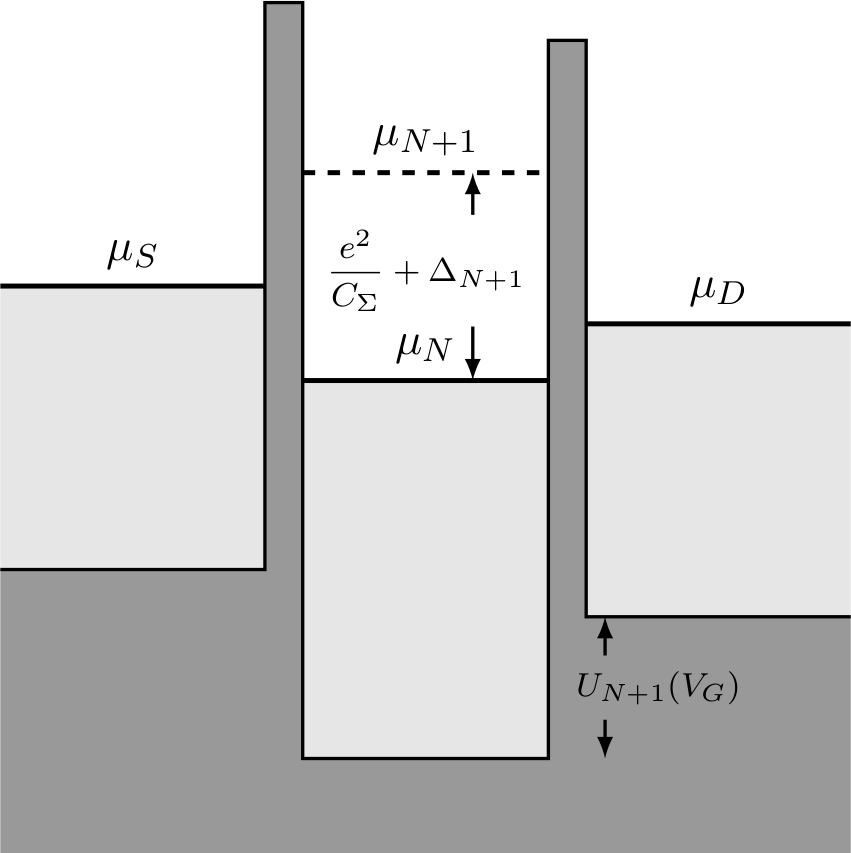
\includegraphics[width=0.6\textwidth]{SET_a}
	\end{figure}	
	
	\note{
		Let's see what happens in terms of the electrochemical potential.
		
		$\mu_N<\mu_D$: the transport is blocked due to the Coulomb blockade. The number of electrons inside the dot is $N$.
	}	
	
\end{frame}

\begin{frame}{Band diagram}

	\begin{figure}
		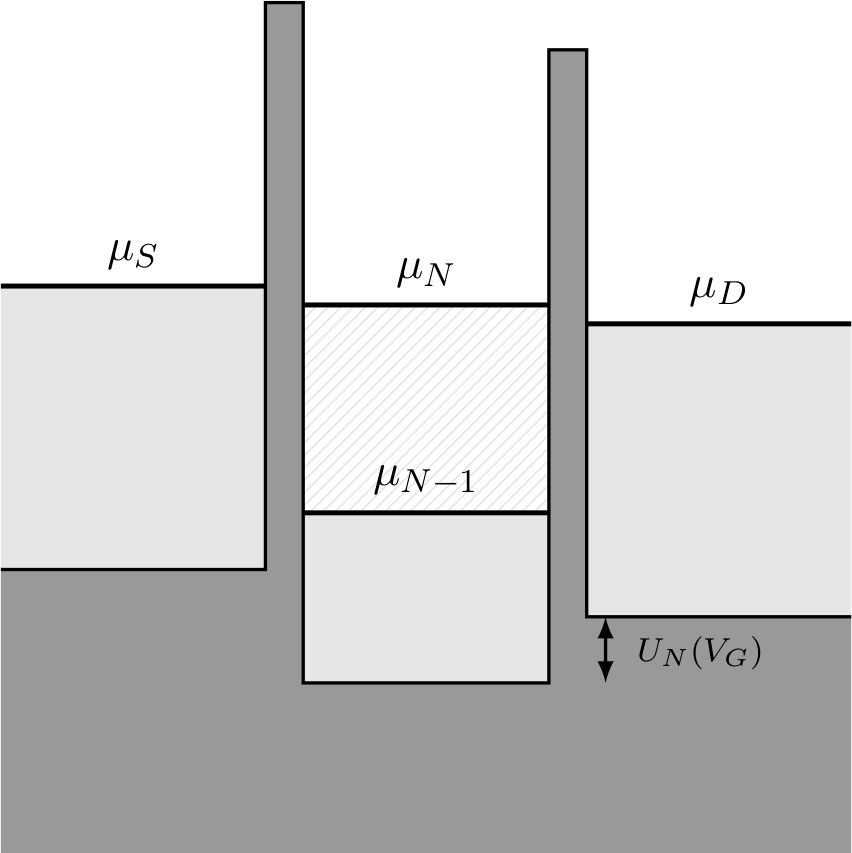
\includegraphics[width=0.6\textwidth]{SET_b}
	\end{figure}	
	
	\note{
		$\mu_S \gtrsim \mu_N \gtrsim \mu_D$: one electron can tunnel the barrier. The number of electrons inside the dot varies from $N-1$ to $N$. This configuration is obtain by lowering $V_G$, in order to increase $\mu_N$.
	}
	
\end{frame}

\begin{frame}{Band diagram}

	\begin{figure}
		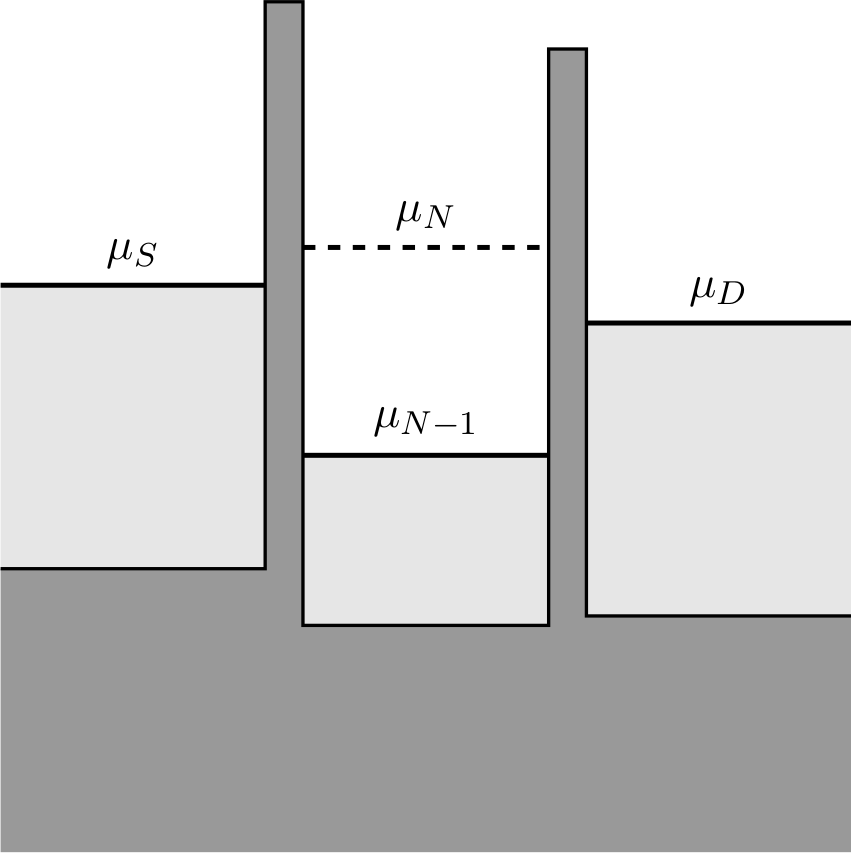
\includegraphics[width=0.6\textwidth]{SET_c}
	\end{figure}	
	
	\note{
		$\mu_N>\mu_S$: the transport is blocked again due to the Coulomb blockade. The number of electrons inside the dot is $N-1$. This situation is obtained by further lowering $V_G$.
	}
	
\end{frame}

\section{The algorithm}

\begin{frame}{The variational principle}
	
	The \alert{variational principle} is a powerful tool that allows, for \emph{any} system, to calculate an \emph{upper bound} estimate for the \emph{ground state} energy.
	
	Being $E_{\text{gs}}$ the ground-state energy, $\Ket{\psi}$ a state whatsoever and $\hat{H}$ the Hamiltonian of the system, the principle states that
	
	\begin{equation}
		E_{\text{gs}} \leq \frac{\Braket{\psi|\hat{H}|\psi}}{\Braket{\psi|\psi}}.
	\end{equation}
	
	We are going to use this principle by calculating the quantity on the right hand side, for a chosen \emph{trial wave-function} $\psi_T$. We will come back later on how to guess a realistic $\psi_T$.
	
\end{frame}

\begin{frame}{The local energy}
	
	In the function-representation of the states, we can recast the above relation as
	
	\begin{equation}
		E_{\text{gs}}
		\leq \int d\vec{\tau}\,\mathcal{P}(\vec{\tau})E_L(\vec{\tau})
		\simeq \frac{1}{n}\sum_{i=1}^{n}E_L(\vec{\tau}),
	\end{equation}
	
	where
	
	\begin{equation}
		\mathcal{P}(\vec{\tau}) = \frac{|\psi_T|^2}{\int d\vec{\tau} \, |\psi_T|^2}
		\qquad
		\text{and}
		\qquad
		E_L(\vec{\tau}) = \frac{1}{\psi_T} \hat{H} \psi_T.
	\end{equation}
	
	The quantity $E_L$ is called the \alert{local energy}.
	
	\note{I dunno anything, fuck yeah!}

\end{frame}

\begin{frame}{The local energy}
	
	\uncover<+->{Let's do a brief recap.}
	
	\begin{itemize}[<+->]
		\item Our upper bound is given by $\int d\vec{\tau}\,\mathcal{P}(\vec{\tau})E_L(\vec{\tau})$
		\item We can calculate it as $\frac{1}{n}\sum_{i=1}^{n}E_L(\vec{\tau})$ for a big enough $n$
		\item In other words, the idea is to sample tons of $E_L$ values at different positions in space and then take the mean
		\item Since the $E_L$'s have a certain distribution, we should sample more points where the probability is higher and less points where the probability is lower, in order to be sure to have a consistent set of samples.
		\item \alert{But how can we achieve such a distribution of samples?}
	\end{itemize}
	
\end{frame}

\begin{frame}{The Metropolis algorithm}

	The solution is to use the \alert{Metropolis algorithm}.
	
	Let's suppose that we have just sampled $E_L$ at a certain point in space, let's call it $\vec{r}^{\text{old}}$. Then, we make a \alert{random move} to another point in space, $\vec{r}^{\text{new}}$.
	
	To check whether we moved to a higher probability region, we calculate the ratio of the respective probabilities, that is 
	
	\begin{equation}
		R 
		\doteqdot \frac{\mathcal{P}(\vec{r}^{\text{new}})}{\mathcal{P}(\vec{r}^{\text{old}})}
		= \frac{|\psi(\vec{r}^{\text{new}})|^2}{|\psi(\vec{r}^{\text{old}})|^2}.
	\end{equation}
	
\end{frame}

\begin{frame}{The Metropolis algorithm}
	
	Then
	
	\begin{itemize}[<+->]
		\item If $R \geq 1$, we accept this move because we are moving to a higher probability region and we sample $E_L$ in the new position.
		\item If $R < 1$, we can't blindly reject this move just because we are moving to a lower probability region; after all, we also have to populate the tails of the distribution! However, we can't accept all of this kind of moves.
	\end{itemize}
	
	\uncover<+->{\emph{Solution}: generate a random number $r \in (0,1)$, and accept the move (i.e., sample $E_L$) if $r \leq R$. Otherwise, the sample is rejected.}
	
	\uncover<+->{This procedure is known as the \alert{brute force} Metropolis algorithm.}

\end{frame}

\begin{frame}{The Metropolis algorithm}
	
	\uncover<+->{Let's recap it:}
	
	\begin{itemize}[<+->]
		\item Choose a starting position $\vec{r}^{\text{old}}$ and a step-length $l$.
		\item Generate a random number $\varepsilon$ in the interval $(0,1)$ and compute a new position $\vec{r}^{\text{new}} = \vec{r}^{\text{old}} + l\varepsilon$.
		\item Compute the acceptance ratio $R = \frac{|\psi_T(\vec{r}^{\text{new}})|^2}{|\psi_T(\vec{r}^{\text{old}})|^2}$.
		\item Generate a new random number $r$ in the interval $(0,1)$.
		\item If $R \geq r$, accept the step and store the position by letting $\vec{r}^{\text{old}} = \vec{r}^{\text{new}}$.
		\item If $R < r$, reject the step and  discard the position by letting $\vec{r}^{\text{new}} = \vec{r}^{\text{old}}$.
	\end{itemize}
	
\end{frame}

\begin{frame}{Choose the proper step-length}

	\uncover<+->{\alert{Problem:}} \uncover<+->{we have \emph{no rule} to say what a proper step length should be.}
	
	\begin{itemize}[<+->]
		\item If it's \emph{too much}, our walker will make huge jumps all around and will sample very few points inside our distribution; the measurement will not be good.
		\item If it's \emph{too less}, our walker will wander around the starting point and will not cover all the distribution space; the measurement will not be good as well.
	\end{itemize}
	
	\uncover<+->{\alert{Solution:}} \uncover<+->{as a \emph{rule of thumb}, one can test different step lengths and then choose the one that gives an acceptance of around $\SI{50}{\percent}$.} 

\end{frame}

\begin{frame}{Importance sampling}

	\uncover<+->{A clever approach is to implement the \alert{importance sampling.}}
	
	\uncover<+->{\emph{Idea:} use the knowledge about the system to improve the acceptance ratio $R$.}
	
	\note{An improved acceptance ratio wastes less points.}
	
	\uncover<+->{Procedure:}
	\begin{itemize}[<+->]
		\item Recast the Schr\"{o}dinger equation a \emph{diffusion problem}, in which the walker is pushed in those regions where the trial wave-function is larger.
		\item The force $\vec{F}$ responsible for pushing the walker is called the \emph{quantum force}, and can be expressed as
		\uncover<+->{
			\begin{equation}
				\vec{F}=2\frac{1}{\psi_T}\nabla\psi_T
			\end{equation}
		}
	\end{itemize}

\end{frame}

\begin{frame}{Importance sampling}

	\begin{itemize}[<+->]
		\item The new position is calculated as
		\uncover<+->{
			\begin{equation}
				r^{\text{new}} = r^{\text{old}} + D\vec{F}(r^{\text{old}})\Delta t + \varepsilon,
			\end{equation}
		}
		\uncover<+->{where $\Delta t$ is a chosen time-step and $D=0.5$ is the diffusion constant.}
		\item The improved acceptance ratio can be expressed as
		\uncover<+->{
			\begin{equation}
				R = \frac{|\psi_T(r^{\text{new}})|^2G(r^{\text{old}},r^{\text{new}},\Delta t)}{|\psi_T(r^{\text{old}})|^2G(r^{\text{new}},r^{\text{old}},\Delta t)}.
			\end{equation}
		}
		\uncover<+->{where $G(x,y,\Delta t)$ is the Green's function}
		\uncover<+->{
			\begin{equation}
				G(y,x, \Delta t) = \dfrac{1}{(4 \pi D \Delta t)^{3N/2}} \exp(-(y - x - D \Delta t F(x))^2 / 4 D \Delta t).
			\end{equation}
		}
	\end{itemize}
	
	\note{
		Here, the random variable $\varepsilon$ is no more uniform! For importance sampling, it's a \emph{Gaussian} random variable.
	}

\end{frame}

\section{The 2-electrons system}

\begin{frame}{The unperturbed system}

	\uncover<+->{Hamiltonian of the system:}
	
	\uncover<+->{
		\begin{equation}
			\hat{H}_0 = 
			\sum_{i=1}^{2} \left( -\frac{1}{2}\nabla_i^2 + \frac{1}{2}\omega^2r_i^2 \right),
		\end{equation}
	}
	
	\uncover<+->{Energy of a single electron in a 2D harmonic potential:}
	
	\uncover<+->{
		\begin{equation}
			E_{s} = \hbar\omega(n_x+n_y+1).
		\end{equation}
	}
	
	\note{
		We begin with the unperturbed Hamiltonian, without the electron-electron repulsion.
		
		Unlike the one-dimensional case, for two dimensions we need two quantum numbers: $n_x$ and $n_y$ for the $x$ and $y$ directions, respectively. This causes a degeneracy in the energy levels. The principal quantum number is $n=n_x+n_y$.
	}

\end{frame}

\begin{frame}{The unperturbed system}
	
	\uncover<+->{Configuration:}
	
	\uncover<+->{
		\begin{figure}
		\centering
		\definecolor{myblue}{rgb}{0,0.447,0.741}	
		\begin{tikzpicture}
			\tikzset{>=latex}
			\draw [ultra thick] (-1,0) -- (1,0) node[midway,below,align=center] {\scriptsize $n_x=0$ \\ \scriptsize $n_y=0$};
			\draw [very thick, myblue, ->] (-0.5,-0.5) -- (-0.5,0.5);
			\draw [very thick, myblue, ->] (0.5,0.5) -- (0.5,-0.5);
		\end{tikzpicture}
		\end{figure}
	}
	
	\uncover<+->{Ground-state energy of the system, in natural units:}
	
	\uncover<+->{
		\begin{equation}
			E_{\text{gs}}=2\omega.
		\end{equation}
	}
	
	\uncover<+->{Exact wave-function:}
	
	\uncover<+->{
		\begin{equation}
			\phi(\vec{r}_1,\vec{r}_2) = C \exp\left(-\omega\left(r_1^2 + r_2^2\right)/2\right).
		\end{equation}
	}

	\note{
		The factor 2 in the ground-state energy stems from the fact that we have two particles in the ground state (spin degeneracy).
		
		$C$ is a normalization constant.
	}
	
\end{frame}

\begin{frame}{The unperturbed system}
	
	\uncover<+->{Since we know the exact wave-function, the problem is trivial. We choose our trial wave-function as}
	
	\uncover<+->{
		\begin{equation}
			\psi_T(\vec{r}_1,\vec{r}_2) = \exp\left(-\alpha\omega\left(r_1^2 + r_2^2\right)/2\right).
		\end{equation}
	}
	
	\uncover<+->{where $\alpha$ is a \alert{variational parameter}.}
	
	\uncover<+->{For $\alpha=1$ we expect to obtain a variational energy \alert{exactly} equal to the ground state energy $E_{\text{gs}}=2\omega$.}
	
	\note{
		In other words, for $\alpha=1$ the upper bound given by the variational principle coincides with the \emph{true} ground state energy.
	}
	
\end{frame}

\begin{frame}{$\omega=1$}
	
	\begin{figure}
		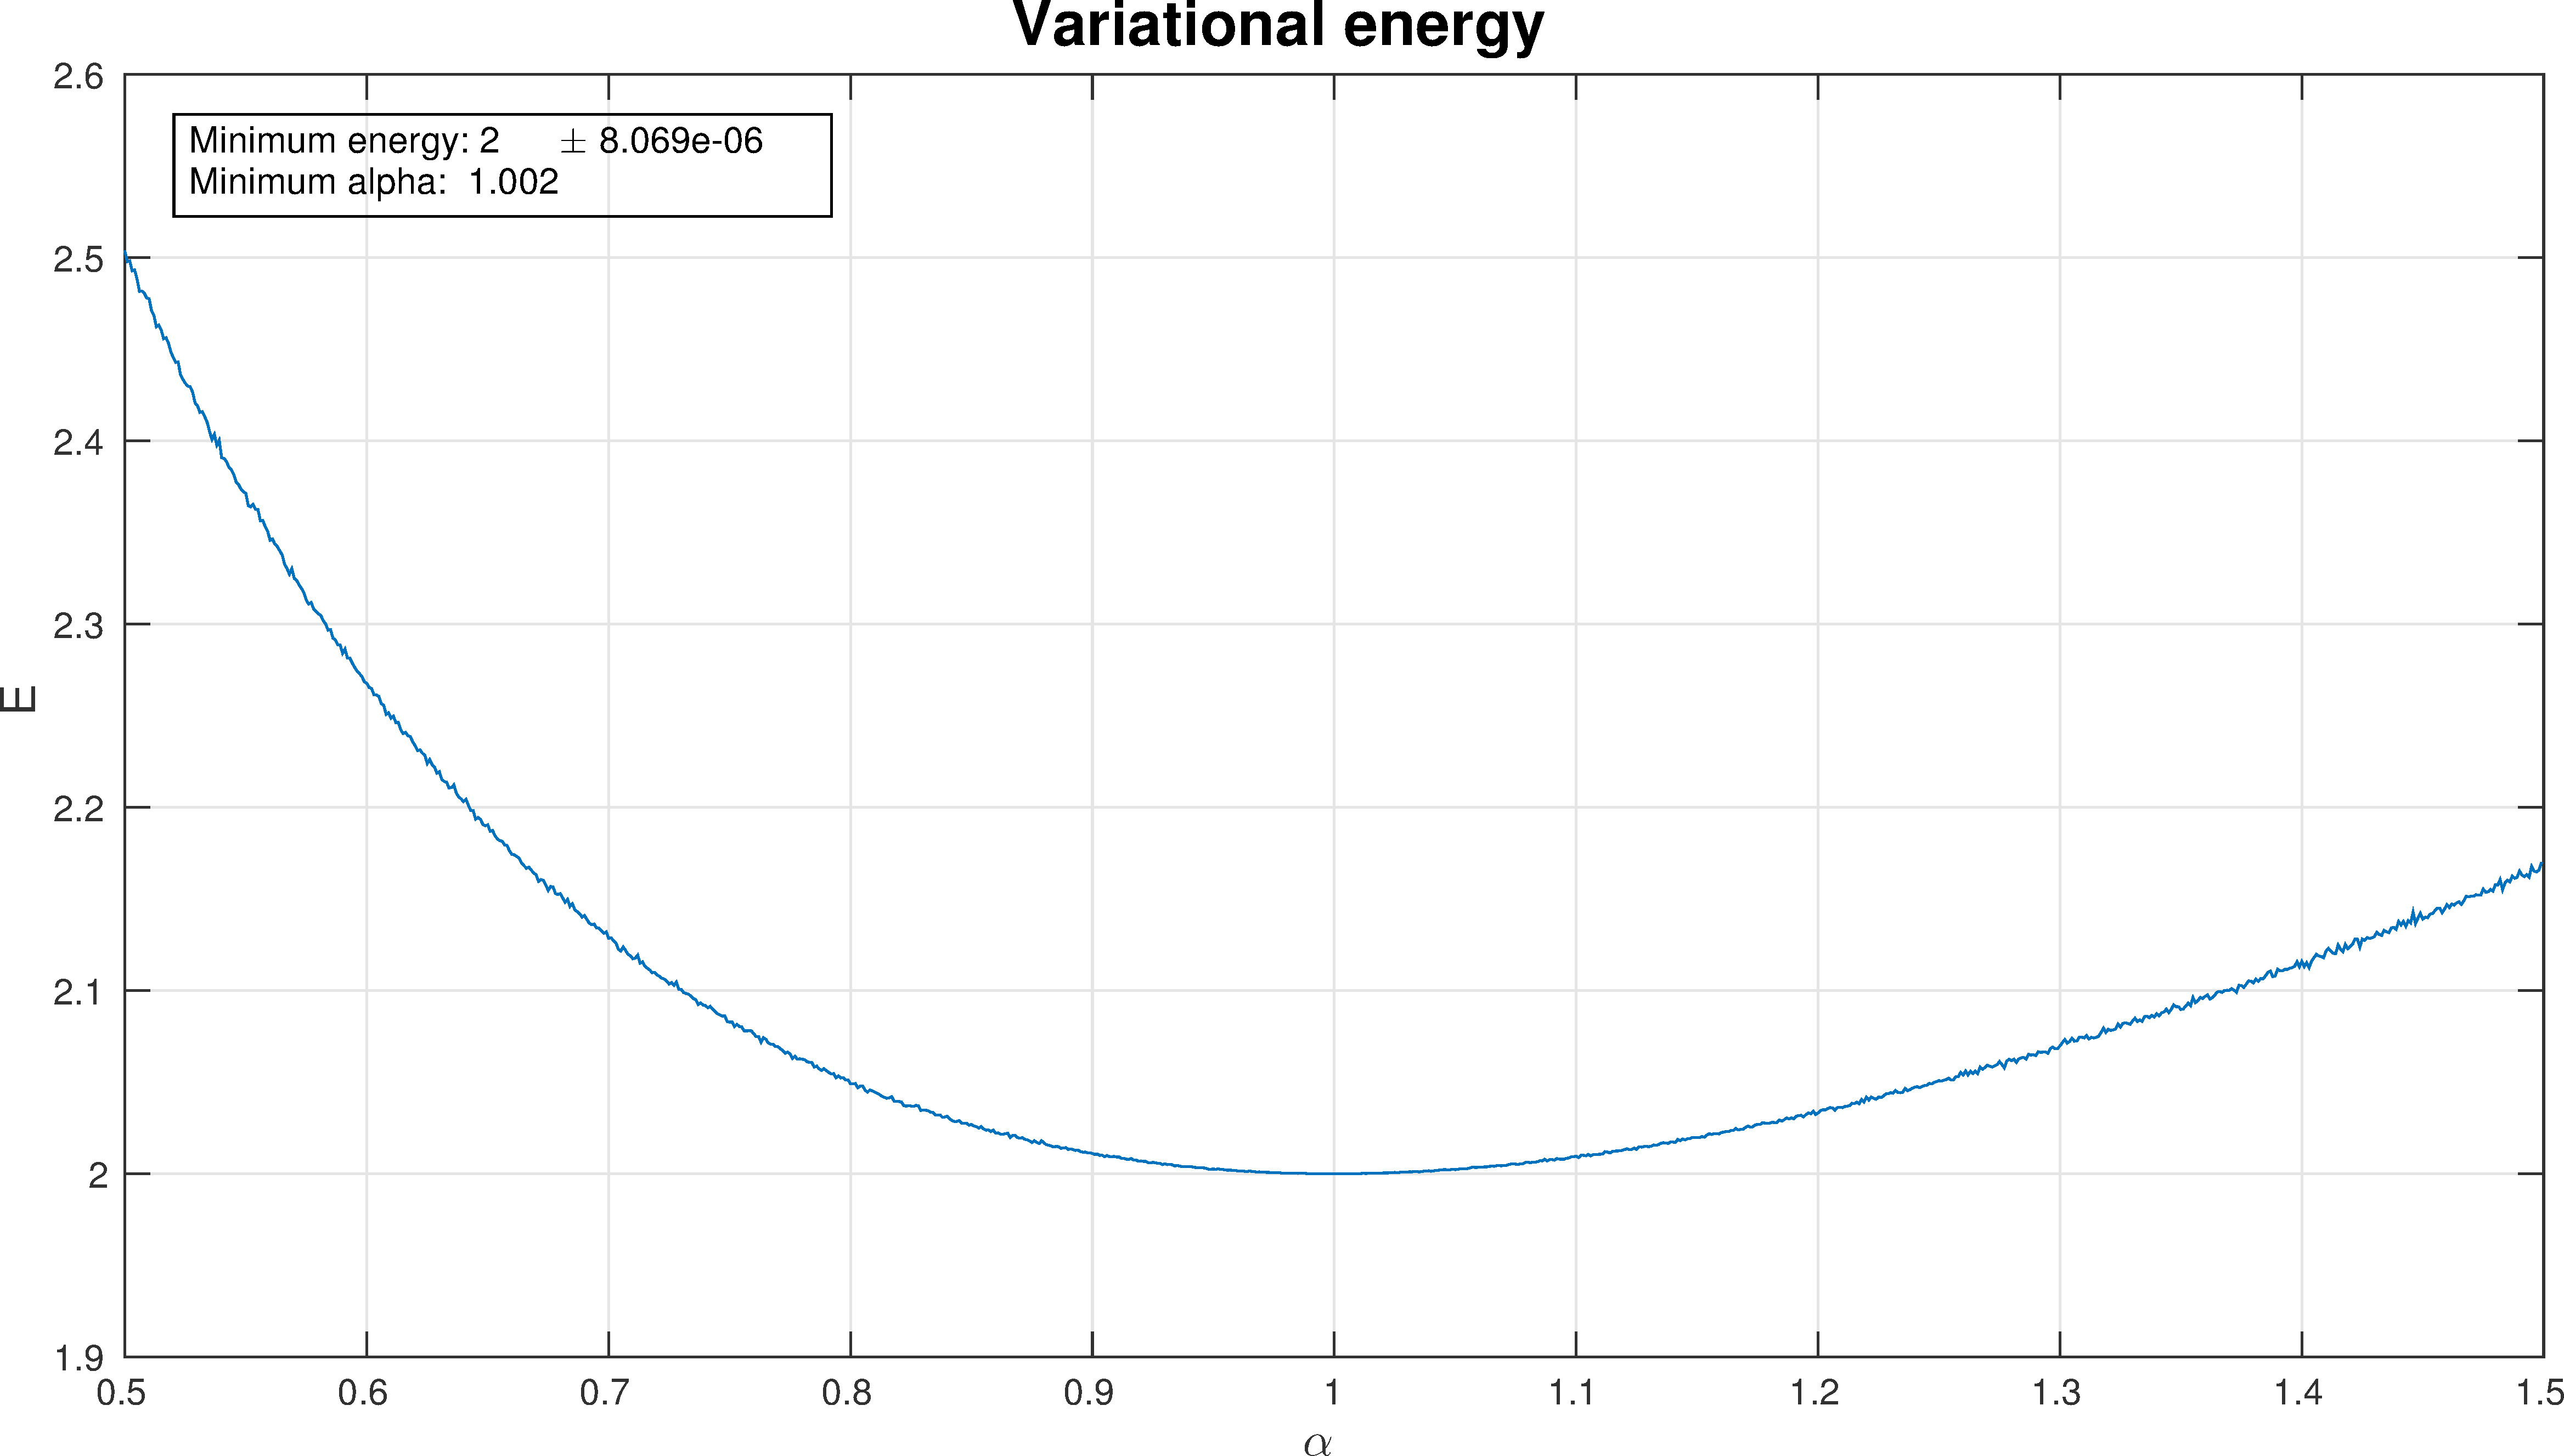
\includegraphics[width=\textwidth]{2e-norep}
	\end{figure}
	
	\note{
		The variational energy versus the variational parameter $\alpha$. The settings used are: brute force sampling with step length 2, no Jastrow factor, no parallelization, $1000$ variations of $\alpha$ around $1$ with step $0.001$, $\SI{1e7}{}$ Monte Carlo steps. Acceptance ratio varies from $40$ to $\SI{60}{\percent}$.
	}	
	
\end{frame}

\begin{frame}{The complete system}

	\uncover<+->{The full Hamiltonian is}
	
	\uncover<+->{
		\begin{equation}
			\hat{H}=-\frac{1}{2} \nabla^2_1 - \frac{1}{2} \nabla^2_2+\frac{1}{2}\omega r_1^2+\frac{1}{2}\omega r_2^2+ \frac{1}{|\vec{r_1}-\vec{r_2}|}.
		\end{equation}			
	}
	
	\uncover<+->{\alert{Problem:}} \uncover<+->{the term
	\begin{equation}
		\frac{1}{|\vec{r_1}-\vec{r_2}|}
	\end{equation}
	could be a division by zero.
	}
	
	\uncover<+->{\emph{Solution:}} \uncover<+->{add, in the wave-function, a factor that cancels the divergence in the Hamiltonian.}	
	
\end{frame}

\begin{frame}{The complete system}
	
	\uncover<+->{The extra factor is usually modeled as}
	
	\uncover<+->{
		\begin{equation}
			\exp\left( \frac{ar}{(1+\beta r)} \right)
		\end{equation}
	}
	
	\uncover<+->{that is called the \alert{Padé-Jastrow} factor.}
	
	\uncover<+->{$a$ is a parameter that depends on the spin, while $\beta$ is a \emph{variational parameter}.}
	
	\note{
		In two dimensions
		\begin{equation}
			a = 
			\begin{cases}
				1 & \text{anti-parallel spin} \\
				1/3 & \text{parallel spin}
			\end{cases}
		\end{equation}
	}	
	
\end{frame}





\section{Conclusion}

\begin{frame}{Summary}

	Something to summarize here.

\end{frame}

\plain{Questions?}

\end{document}
